
\section{Producing Detector Inefficiency Corrections} \label{KrypCalCode}

Now that we have related the strength of the field effect in both $^{83m}$Kr S2 and $^{83m}$Kr S1 data to the S1a/S1b ratio we can make use of these relationships to produce detector inefficiency corrections during every $^{83m}$Kr calibration.  This process is very similar to (and in some ways, the reverse of) the process to measure the field effect in $^{83m}$Kr S2 data. Nevertheless, we will describe the process here for completeness and clarity.

\subsection{Mapping S1a/S1b}

For a $^{83m}$Kr calibration at any point in time, we begin by measuring the Z dependence of the S1a/S1b ratio using the methods of section  \ref{section:S1aS1b1} and  \ref{section:S1aS1b2}.  We first divide the detector into drift times bins with a width chosen such that each bin has roughly 300 events.   A Gaussian distribution is fit to the S1a and S1b spectrum of each bin to determine the mean pulse areas versus Z.  A second order polynomial is fit to the ratio of the Gaussian means versus Z and is used to determine the S1a/S1b at any drift time in the detector.  

If the $^{83m}$Kr data set has more than 100,000 S1a/S1b events (after cuts are applied) a three dimensional S1a/S1b map is also constructed. The detector is divided into three dimensional voxels with dimensions chosen such that each voxel has roughly 200 events.  A three dimensional map of S1a/S1b ratio is produced by fitting a Gaussian distribution to the S1a and S1b pulse area spectrum in each voxel.  A spline interpolation is used to determine the S1a/S1b ratio between the three dimensional voxels, and the S1a/S1b Z dependence map is used to extrapolate outside of the range of the voxels. 

\subsection{Removing the field effect from $^{83m}$Kr Data}

We use the $^{83m}$Kr S2 field effect to S1a/S1b relationship and S1 field effect to S1a/S1b relationship measured in sections \ref{section:FieldEffects} and \ref{section:S1relation2} to convert the Z and three dimensional maps of S1a/S1b into measures of the field effects in the S1 and S2 data.  The strength of the field effect is measured by $\frac{S1_E(xyz)}{S1_E(center)}$ and $\frac{S2_E(xyz)}{S2_E(center)}$.  Dividing the raw $^{83m}$Kr data by the strength of the field effect normalizes any field induced recombination variation to the level of recombination that occurred at the center of the detector, at the time the field effect relationships were measured.  This is equivalent to normalizing electric field in the $^{83m}$Kr data to it's value at the center of the detector in September 2015. Applying these normalization factors produces field effect corrected S1$_F$ and S2$_F$ signals, as shown in equations \ref{S1F-2} and \ref{S2F-2}. (Figure \ref{fig:KrypCalLifetime})
\begin{align} 
S1_F &=S1 \times \frac{S1_E(center)}{S1_E(xyz)} \label{S1F-2} \\
S2_F &=S2 \times \frac{S2_E(center)}{S2_E(xyz)} \label{S2F-2}
\end{align}

\subsection{Measuring Detector Inefficiencies}

After removing the field effects from the $^{83m}$Kr data we are ready to measure the residual spatial pulse area variation due to detector inefficiencies alone.  We first measure the Z dependence of the S2$_F$ and S1$_F$ pulse areas by slicing the detector into drift time bins with widths defined such that each bin has roughly 300 events.  A Gaussian distribution is fit to the S2$_F$ and S1$_F$ spectra of each bin to determine the location of the spectra maximums. (Figure \ref{fig:KrypCal_S2ZDep} and Figure \ref{fig:KrypCal_S1ZDep}) In the case of the S2$_F$ signal, a cubic interpolation is used to determine the S2$_F$ Z dependence between each drift time bin, and a linear extrapolation based on the first and last 20\% of Gaussian distribution data points is used to determine the S2$_F$ Z dependence above and below the span of the drift time bins.  A detector inefficiency correction for the Z direction is defined by taking the ratio of the S2$_F$  pulse area at a height of 4 $\mu$seconds (just below the liquid surface) to the S2$_F$ pulse area as a function of Z as described in the equation
\begin{equation}
\epsilon_{(S2,Z)} = \frac{S2_F(z=4)}{S2_F(z)}.
\end{equation} 

In the case of the S1$_F$ signal, a second order polynomial is used to determine the S1$_F$ Z dependence between and outside of each drift time bin. A detector inefficiency correction for the Z direction is defined by taking the ratio of the S1$_F$  pulse area at the center of the detector ($z_c$ as defined by the average drift time of $^{83m}$Kr) to the S1$_F$ pulse area as a function of Z as described in the equation
\begin{equation}
\epsilon_{(S1,Z)} = \frac{S1_F(z_c)}{S1_F(z)}.
\end{equation} 


The XY dependence of the field removed S2$_F$ and S1$_F$ signals are found by dividing the z inefficiency corrected (S2$_F \times \epsilon_{(S2,Z)}$ and S1$_F \times \epsilon_{(S1,Z)}$) data into two dimensional XY bins with lengths defined such that each bin has roughly 300 events, and then fitting Gaussian distributions to the data of each bin.  The mean of the Gaussian distribution from each bin is used to construct S2$_F$ and S1$_F$ XY dependence maps, with a spline interpolation and extrapolation being used to determine the XY dependence between and outside of the bins.  A detector inefficiency correction for the XY direction is defined by taking the ratio of the z inefficiency corrected S2$_F$ (or S1$_F$) pulse area at the center of the detector to the z inefficiency corrected S2$_F$ (or S1$_F$) pulse area as a function of XY in cm, as shown below
\begin{align}
\epsilon_{(S2,XY)} &= \frac{\epsilon_{(S2,Z)} \times S2_F(x_c,y_c,z)}{\epsilon_{(S2,Z)} \times S2_F(xyz)} \\
\epsilon_{(S1,XY)} &= \frac{\epsilon_{(S1,Z)}\times S1_F(x_c,y_c,z)}{\epsilon_{(S1,Z)} \times S1_F(xyz)}.
\end{align} 
where $x_c$ and $y_c$ are the x and y center of the detector in uncorrected coordinates determined by taking the average position of the $^{83m}$Kr events in each direction.  

To apply these S1 and S2 efficiency corrections to data at any time, we must interpolate between the corrections in time.  The S2$_E$ XY, S1$_E$ Z, and S1$_E$ XY efficiency corrections are not expected to change rapidly in time, so a simple nearest neighbor interpolation is used to apply these efficiency corrections to data sets at any point in time.  However, the S2$_E$ Z dependence is expected to change rapidly in time due to the sudden changes in xenon purity introduced by detector operations.  To account for this, we find the $^{83m}$Kr calibration taken immediately before and after a particular data set which the detector efficiency corrections are being applied to.  A weighted average of the $^{83m}$Kr S2$_E$ Z dependence splines, with weights based on the time between each $^{83m}$Kr calibration data set and the data set being corrected, is used to defined a time interpolate S2$_E$ Z dependence correction.  Multiplying the raw S2 and S1 signals of any data set by the time-interpolated Z and the XY correction factors results in inefficiency corrected S2$_E$ and S1$_E$ signals (with field effects still present).
\begin{align}
S2_E &=S2 \times \epsilon_{(S2,Z)} \times \epsilon_{(S2,XY)} \\
S1_E &=S1 \times \epsilon_{(S1,Z)} \times \epsilon_{(S1,XY)}
\end{align}

Note that although XY correction factors were determined for the analysis in reference~\cite{Run4paper}, they were not applied to the data due to complications with extrapolating the correction factors outside of the two dimensional bins.  The XY correction factors only adjust the S1 and S2 signals by a few percent, so the negative impact of occasional erroneous extrapolations outweighed the benefits of applying the XY correction factors.

\section{Evaluating the Signal Corrections} \label{Results}

In this section we will cover a number of metrics which have been used to determine how well the corrections are working in Run04.  A version of the corrections which do not acknowledge the spatial and time dependent field in WS2014-16 (i.e. corrections which have field effects mixed into the $^{83m}$Kr results) have been produced for comparison of each metric. This flawed version of the corrections normalizes the $^{83m}$Kr S1 and S2 signals everywhere in the detector, regardless of whether the variation is induced by field effects or detector inefficiency. 

\subsection{Energy Spectra}\label{Result:Spectra}

The $\chi^2$ method presented in section \ref{section:S1relation2} finds an average total reduced $\chi^2$ of 0.8413 for the CH$_3$T and $^{83m}$Kr energy spectra, with a reduced $\chi^2$ of  150.6/124=1.2143 (p=0.05) for CH$_3$T alone and a reduced $\chi^2$ of 12.17/26=0.4682 (p=0.99) for $^{83m}$Kr alone.  The resulting $^{83m}$Kr energy spectra from September 2015 and February 2016 are shown in figure \ref{Kr2p22_KrE}.  The Gaussian means differ from the expected 41.55 keV by less than one sigma, and the reduced $\chi^2$ based on the Z dependence of the Energy spectra returns a p-value of 0.99.

\begin{figure}
\centering
\subfloat{{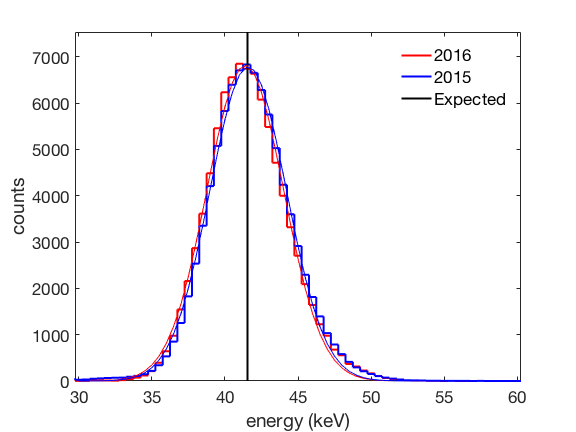
\includegraphics[width=6.5cm]{figures/KrEnergy.png} }}
\qquad
\subfloat{{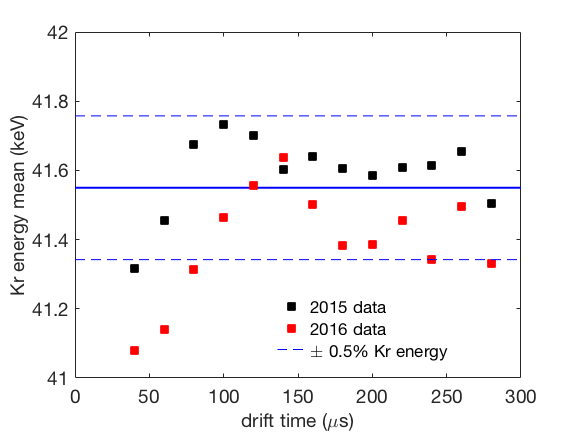
\includegraphics[width=6.5cm]{figures/KrEnergyZDep.png} }}
\caption{ (Left) The energy spectrum of $^{83m}$Kr data in September 2014 (red) and September 2015(blue) after determining the S1 field effect to S1a/S1b relationship from the reduced $\chi^2$ method. The energy spectrum is expected to be a Gaussian distribution centered around the black line.  (Right) The Z dependence of the $^{83m}$Kr energy peaks in September 2014 (red) and September 2015 (black).}
\label{Kr2p22_KrE}
\end{figure}

The CH$_3$T energy spectra from calibrations in September 2014, November 2014, February 2015, September 2015, and February 2016 are shown in figure \ref{Kr2p22_H3E}.  The fractional difference between the expected CH$_3$T spectrum and the CH$_3$T is shown below each energy spectrum.  Fractional residuals of up to 3 $\sigma$ are comparable to our CH$_3$T results from Run03.


\begin{figure}
%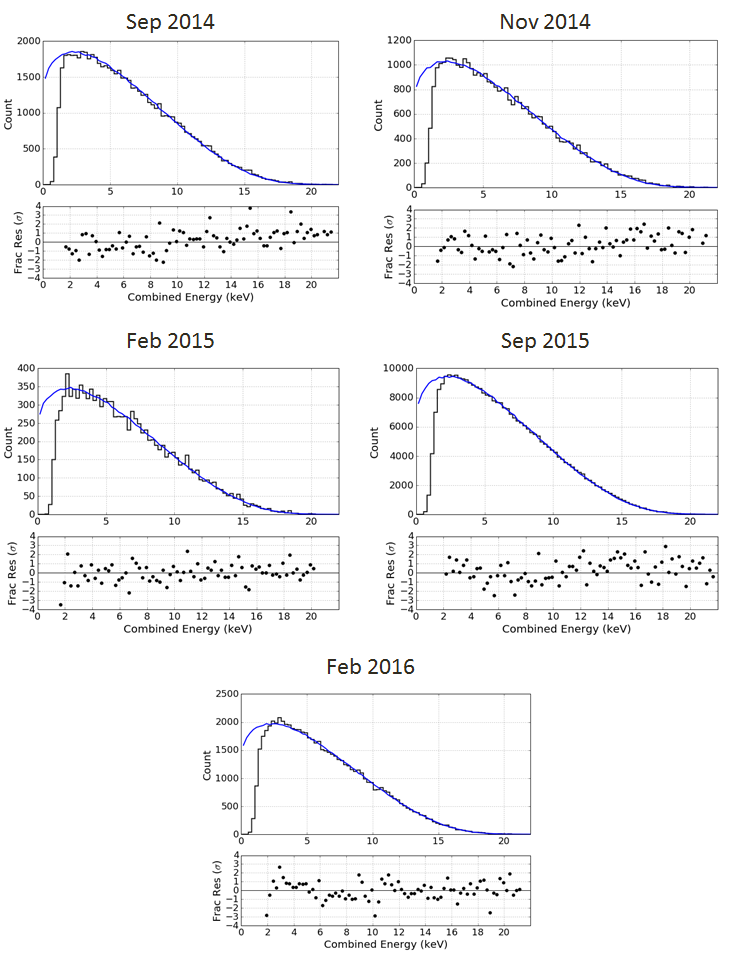
\includegraphics[scale=0.4]{figures/KrypCal_2p22_AllCH3TEnergy.png}
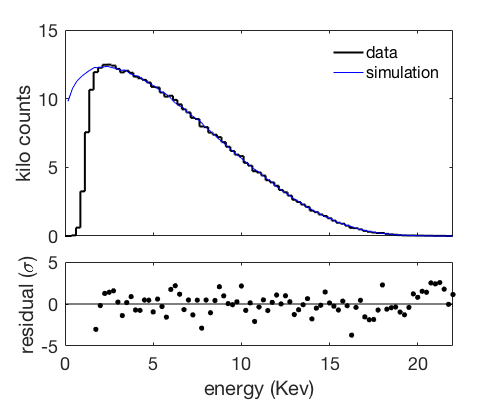
\includegraphics[scale=0.4]{figures/CH3T_energy_wres_sep2015.png}
\captionof{figure}{The September 2015 CH$_3$T energy spectra resulting from KrypCal corrections.}
 \label{Kr2p22_H3E}
\end{figure}


A version of the corrections which do not acknowledge the spatial and time dependent field in WS2014-16 returns best fit values of $g_1=0.100 \pm 0.001$ and extraction efficiency of EE$=1.08 \pm 0.030$.  This optimal value of the extraction efficiency is 40\%-80\% higher than our expectations based on Guschin data and our extraction field strength, and exceeds 100\% (Figure \ref{EEexpec}).  The $^{83m}$Kr and CH$_3$T energy spectra also produce an worse average reduced $\chi^2$ of 1.12 for the $^{83m}$Kr and CH$_3$T energy spectra when compared to the expected energy spectra, with a reduced $\chi^2$ of 10.06/26=0.3869 for $^{83m}$Kr alone, and a reduced $\chi^2$ of 230.2/124=1.8562 for CH$_3$T alone. 

\subsection{G1 and EE}

The $\chi^2$ method presented in section \ref{section:S1relation2} finds best fit values of $g_1=0.098 \pm 0.001$ and $EE=0.808 \pm 0.029$.  This is consistent with our expectations of an extraction efficiency between 0.6 and 0.8, based on our extraction field models and the liquid level, and is much better than the $g_1=0.100 \pm 0.001$ and $EE=1.08 \pm 0.030$ result found in section \ref{Result:Spectra}.  Likewise, the best fit value of $g_1$ is within one sigma of our expectation of g$_1$=0.108 $\pm$ 0.010 found in section \ref{G1pred}. 

\begin{center}
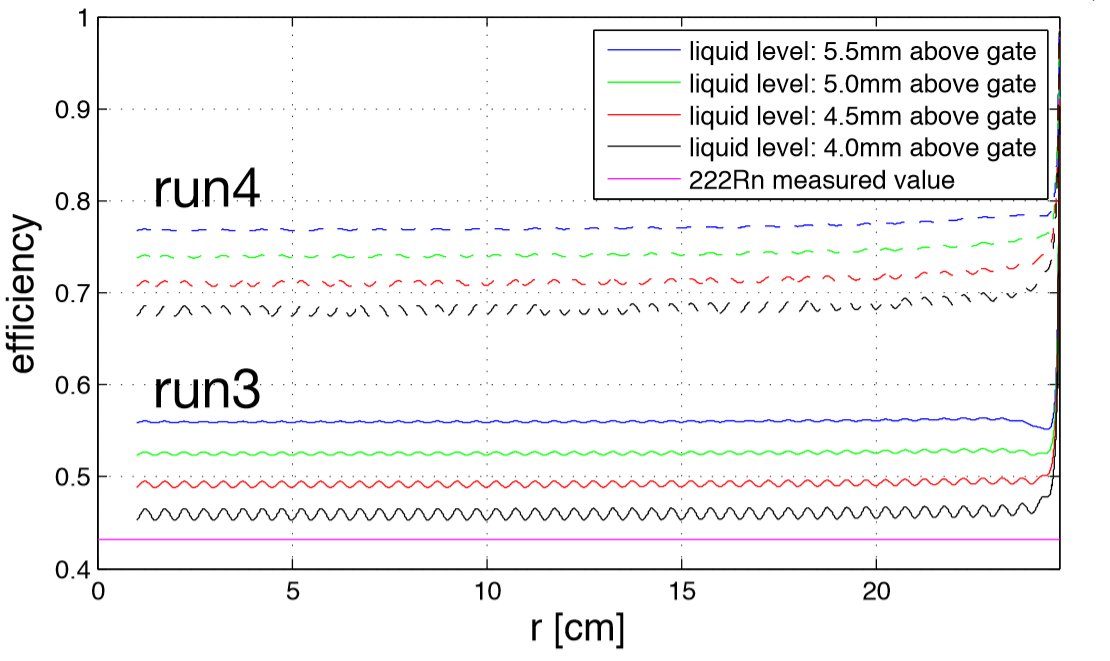
\includegraphics[scale=0.3]{figures/GuschinEE.png}
\captionof{figure}{The expected extraction efficiency based on the electric field map.  The expectation is derived from a Guschin curve, and is dependent on the height of the liquid above the gate.  The exact liquid level is unknown, so a range of possible values is depicted.}
 \label{EEexpec}
\end{center}


\subsection{Lifetime Estimates}

The nonuniform field in the LUX detector produces higher recombination of $^{83m}$Kr events in the bottom of the detector.  This results in an attenuation of the $^{83m}$Kr S2 signal that is directly proportional to drift time.  This effect mimics the attenuation of the $^{83m}$Kr S2 signal produced by impurities capturing charge as it drift to the top of the detector.  As a result, when field effects are not properly accounted for in a $^{83m}$Kr calibration, the electron lifetime is drastically underestimated.  The version of the corrections which does not account for field effects in WS2014-16 measured electron lifetimes below 350 $\mu$seconds at all points in time.  This problem is rectified by the methods presented here, which measure accurately measure the electron lifetime to be as high as a few milliseconds (Figure~\ref{fig:KrypCalLifetime}). The higher values of electron lifetimes have been confirmed by a separate, low energy $^{37}$Ar injection performed at the end of LUX's WS2014-16 data collection.

\begin{center}
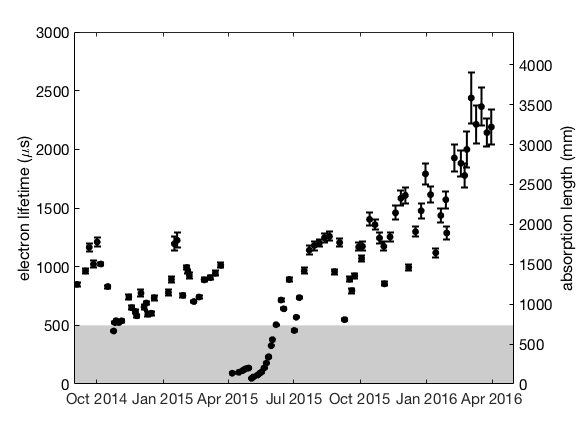
\includegraphics[scale=0.4]{figures/LUX_eLifetime_Kr2p22.png}
\captionof{figure}{The electron lifetime over WS2014-16 found by fitting an exponential to the S2$_F$ Z dependence.  Red areas indicate circulation outages.  At high lifetimes the S2$_F$ Z dependence is less exponential, leading to larger errors on the measurement.}
 \label{fig:KrypCalLifetime}
\end{center}

\subsection{Nuclear Recoil Band}

Nuclear recoils are much less sensitive to field variation effects in the detector, so a significant spatial dependence in the NR band it would indicate a flaw in the corrections. With the methods presented here, LUX's multi-Z NR band calibration in October 2014 shows $\sim4\%$ spatial dependence in the NR band, which is consistent with expectations from NEST (Figure \ref{NRBandZ}) . The result of the same calibration using a version of the corrections which do not properly account for field effects is also shown in Figure \ref{NRBandZ}.  The underestimate of the electron lifetime and subsequent over correction of the S2 data produces a large, non-physical z dependence in the NR band when field effects are not accounted for.  

\begin{figure}
\centering
\subfloat{{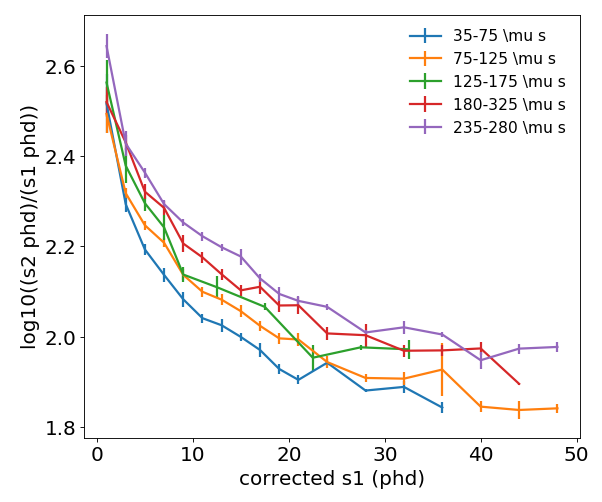
\includegraphics[width=6.5cm]{figures/NRband_run3.png} }}
\qquad
\subfloat{{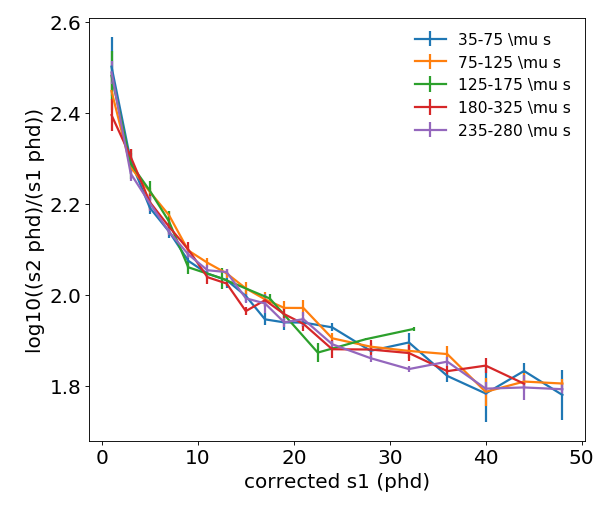
\includegraphics[width=6.5cm]{figures/NRband_run4.png} }}
\caption{ (Top) The Z dependence of the NR band mean using a version of KrypCal which does not properly account for field effects. (Bottom) The Z dependence of the NR band mean from the same datasets using a version of KrypCal which does properly account for field effects.  }
\label{NRBandZ}
\end{figure}

\subsection{Electron Recoil Band}

The electron recoil band that results from the corrections which do account for field effects should have significant spatial and time dependence due to the recombination variation induced by the nonuniform electric field remaining in the data. The corrected ER band calibration data from September 2015 was divided into three dimensional voxels with a height of 86 $\mu$seconds and an X and Y width of 16 cm.  We see a 16\% spatial variation of the ER band in September 2015 (at S1=20 phd), which is comparable to the libNEST prediction of a 13\% spatial variation (at S1=20 phd).  We also observe a $\sim$1\% variation in time for the total ER band over the duration of WS2014-16 (Figure \ref{ERBandVariation}). The relative size of the spatial and time dependence of the ER band is consistent with expectations, since the spatial dependence of the electric field is stronger than the time dependence of the electric field. 

%The spatial variation quoted is measured at S1c=20 phd

\begin{figure} 
\centering
\subfloat{{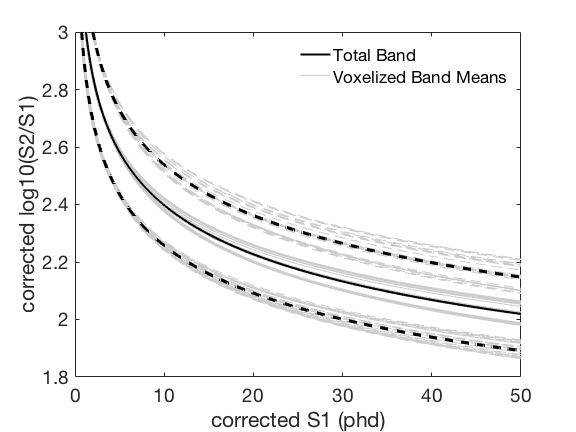
\includegraphics[width=6.5cm]{figures/Sep2015_VoxelizedBands_WithUpperLower.png} }}
\qquad
\subfloat{{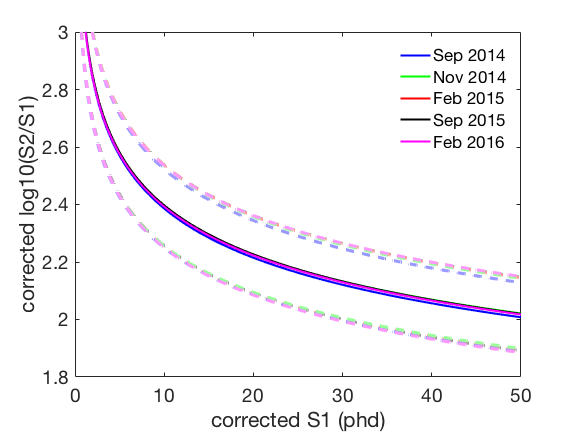
\includegraphics[width=6.5cm]{figures/OverlayOfAllERBands.png} }}
\caption{ (Left) The spatial variation of the KrypCal corrected ER band from September 2015.  The black band represents the total, unbinned ER band and the grey bands represent the ER band from each voxel. (Right) The time dependence of the total, unbinned ER band as measured by the KrypCal corrected data at four points in time.}
\label{ERBandVariation}
\end{figure}

Further evidence that the corrections are behaving properly appears in the ER band's electric field dependence.  We fit a power low to the ER band in September 2015 and relate the fit parameters to the S1a/S1b ratio.  We observe the polynomial relationships shown in Figure~\ref{ERBand_S1aS1bToER}.  These measured relationships can be used to reconstruct the ER band from any of the seven tritium calibrations that were acquired during Run04, from measurements of S1a/S1b alone.  Each of the reconstructed bands are within 3\% of the measured the ER bands, with p-values close to 1 in all cases.  

Figure~\ref{Feb2016ERPred} shows the close agreement between the ER band predicted from the polynomial relationships shown in Figure~\ref{ERBand_S1aS1bToER} to the ER band measured in data.  The predicted ER band was produced prior to measurement of the ER band in data.  Although not shown, the spatial dependence of the ER band is also reproduced within 2\% of the measured band. 

\begin{figure} 
\centering
\subfloat{{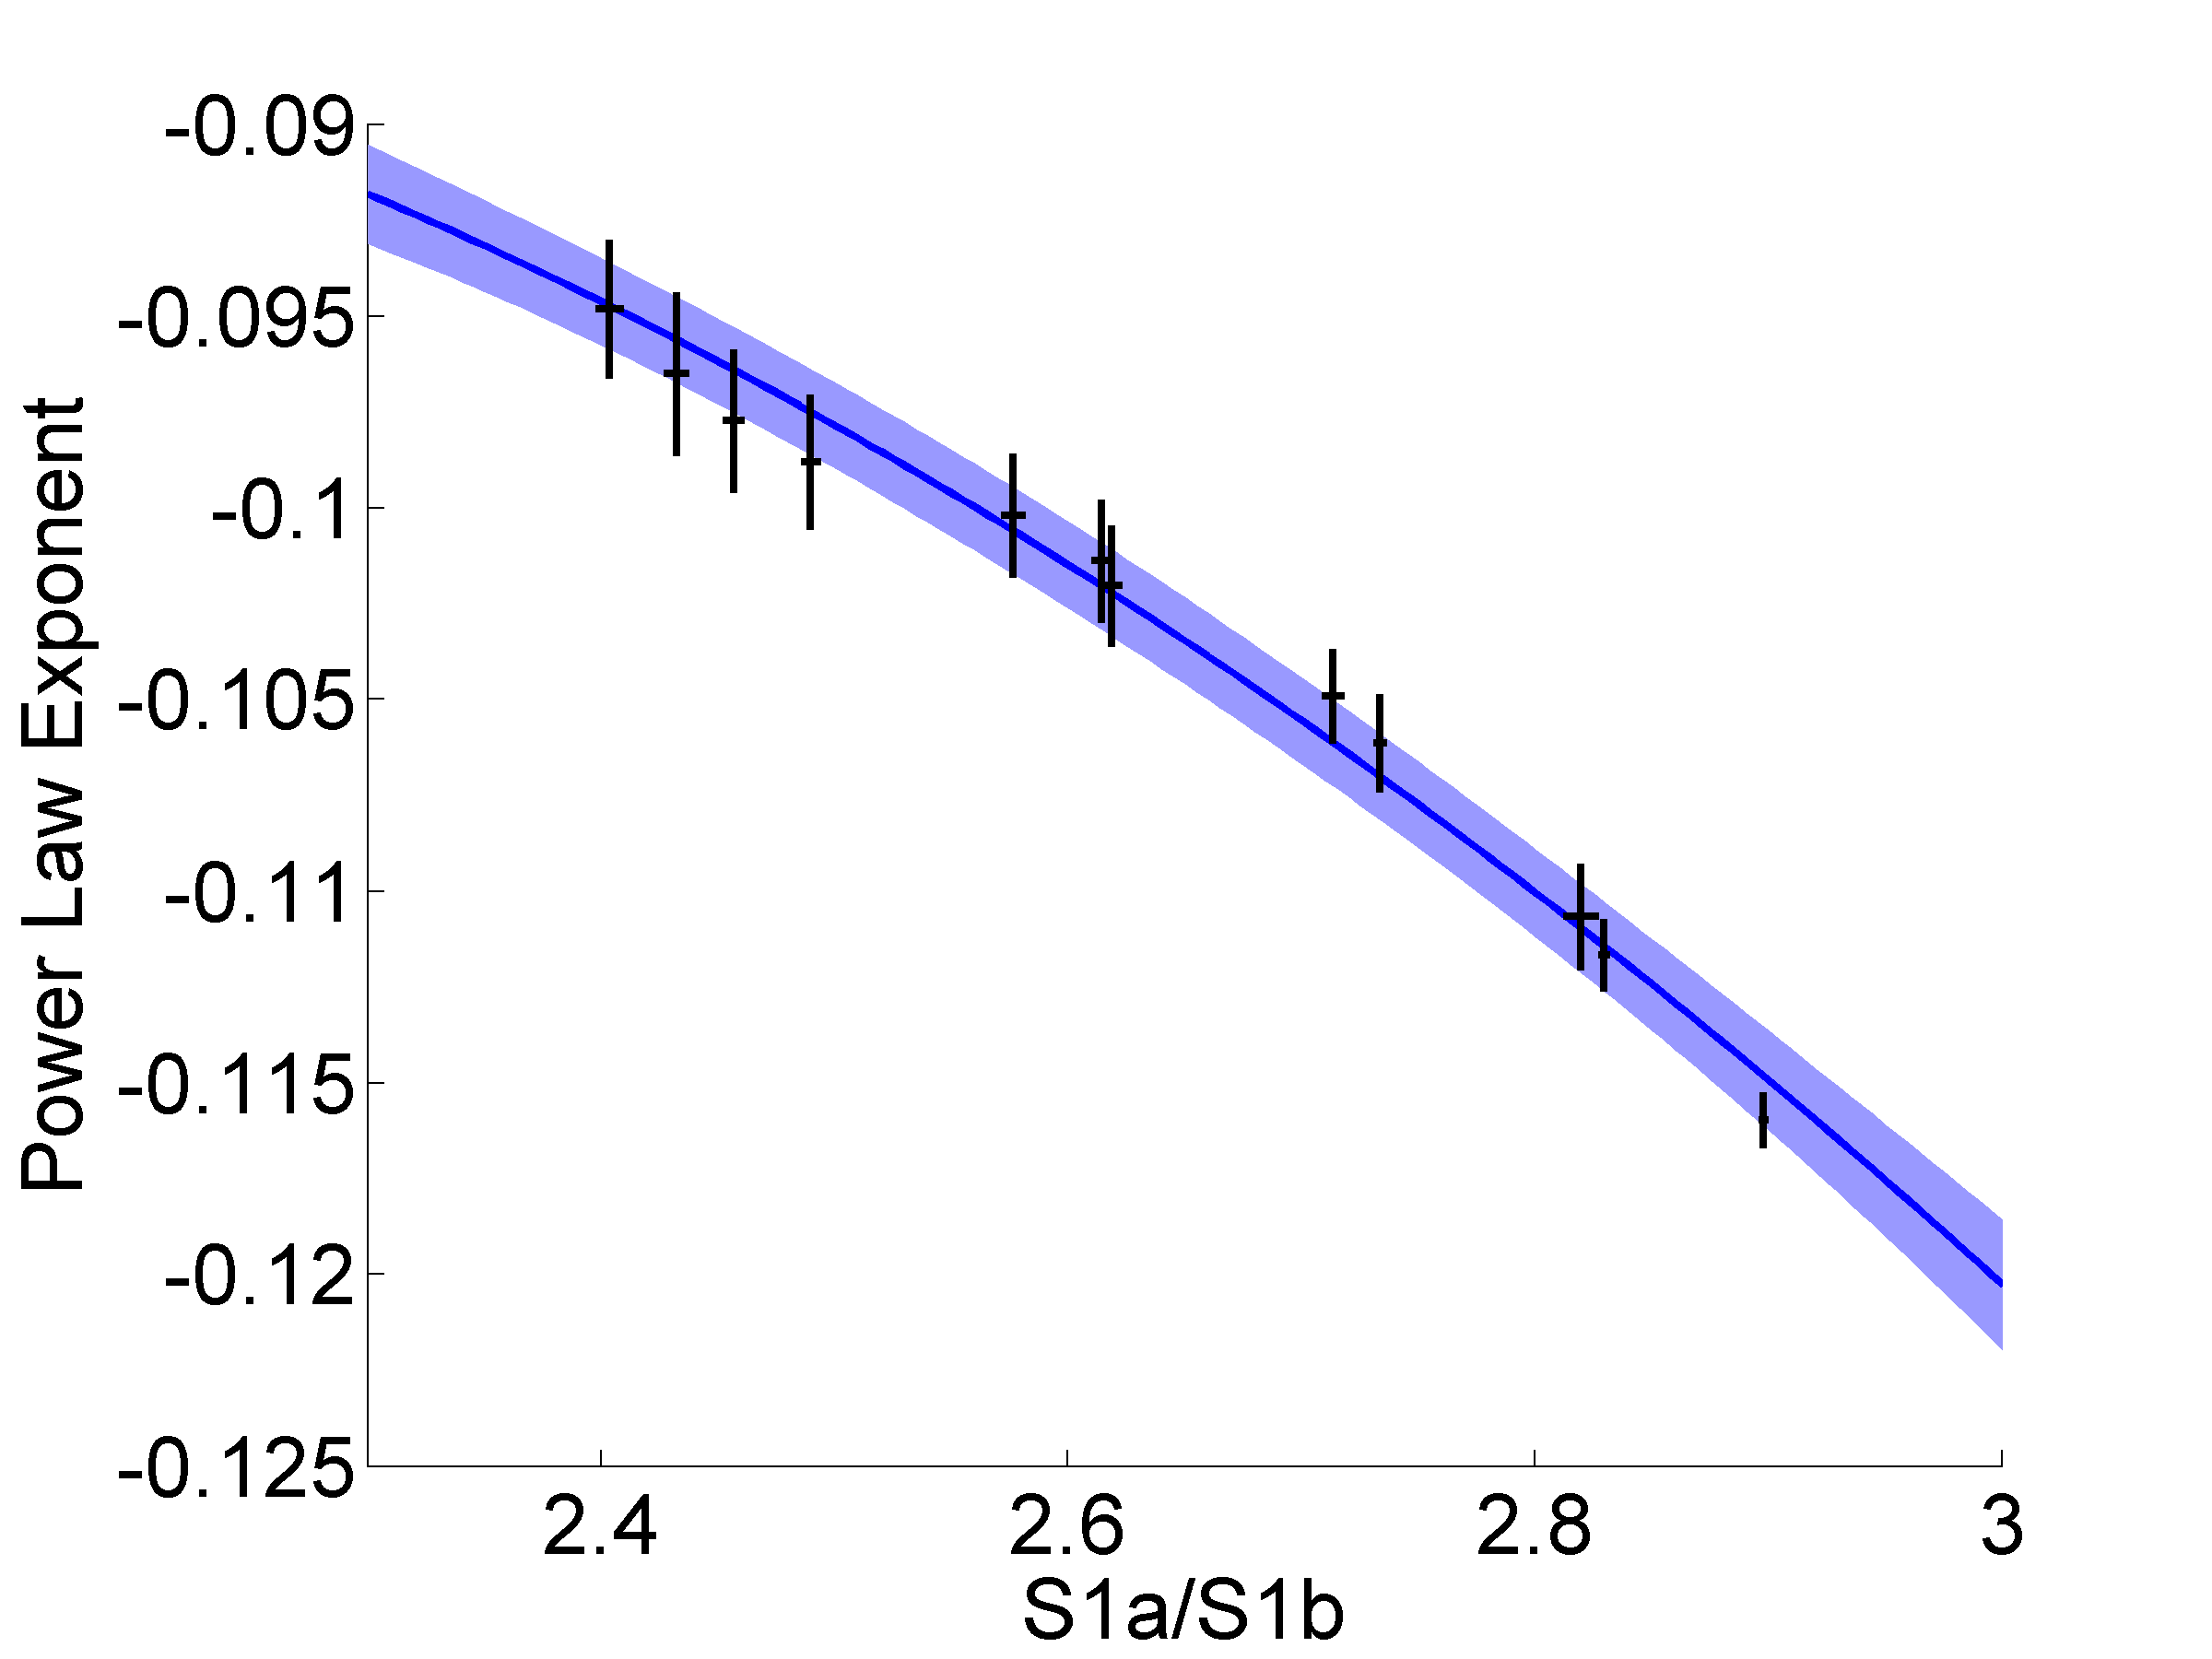
\includegraphics[width=6.5cm]{figures/PowerLawExponent.png} }}
\qquad
\subfloat{{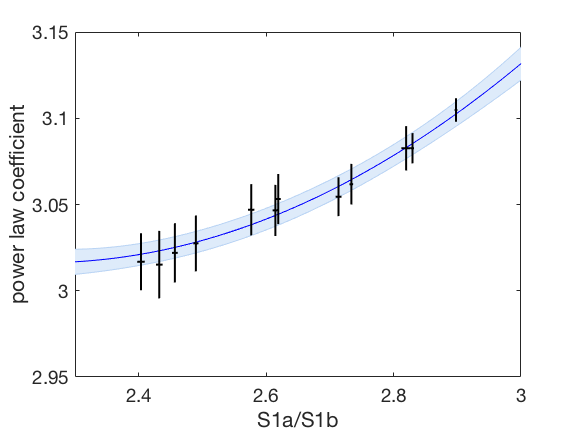
\includegraphics[width=6.5cm]{figures/PowerLawCoefficient.png} }}
\caption{ (Left) The measured relationship between S1a/S1b and the ER band power law exponent. (Right) The measured relationship between S1a/S1b and the ER band power law coefficient. The light blue region indicates one $\sigma$ uncertainties on each fit.}
\label{ERBand_S1aS1bToER}
\end{figure}


\begin{center}
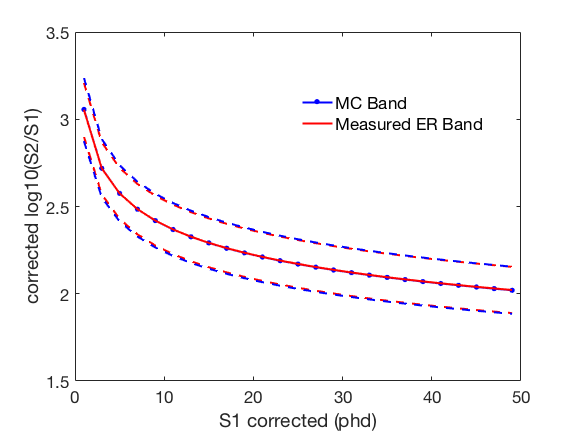
\includegraphics[scale=0.45]{figures/Feb2016_ERPrediction.png}
\captionof{figure}{Monte Carlo data for the February 2016 ER band generated from S1a/S1b using the relationship found in Figure \ref{ERBand_S1aS1bToER}.  A fit to the Monte Carlo data is shown in blue, and a fit to the actual calibration data (not shown) is shown in red.}
 \label{Feb2016ERPred}
\end{center}
